In this section, the basic GeoPAT procedures are presented: 

\begin{itemize}
	\item {\bf Search} - search for areas similar to a query
	\item {\bf Change detection} - comparison of local patterns between two maps
	\item {\bf Segmentation} - division of a map into regions of cohesive patterns
	\item {\bf Clustering} - grouping patterns that are similar to each other
\end{itemize}

The procedures are explained using several workflow schemes and examples.
The examples how to process categorical data are shown on a $42\times 69$ km ($1400\times 2300$ px) part of the National Land Cover Dataset (NLCD) covering area around the city of Augusta, GA (Figure \ref{FIG:AUGUSTA}).
This area is characterized by a high diversity of land cover categories and patterns.
Thus it is perfect for various pattern analyzes.

\begin{figure}[H]
	\centering
	\includegraphics[width=\textwidth]{atlanta.png}
	\caption{Part of NLCD, covering area around Augusta, GA used in the examples}
	\label{FIG:AUGUSTA}
\end{figure}

Examples of time-series analysis are based on monthly sums of precipitation for area of Great Britain from the WorldClim database (\cite{hijmans2005very}; Figure \ref{FIG:PRCP}).
It consists of twelve raster files, where each file has 240 rows and 319 columns.
Precipitation values are expressed in millimeters.

\begin{figure}[H]
	\centering
	\includegraphics[width=\textwidth]{prcp.png}
	\caption{Monthly sums of precipitation for area of Great Britain used in the time-series examples}
	\label{FIG:PRCP}
\end{figure}

\FloatBarrier

\subsection{Search}

Search functionality enables users to produce maps of similarity. 
These maps show the level of similarity between a specified motifel (query) and a grid of motifels.
The input is one or more GeoTIFF raster maps (depending on a data and signature type; see appendix \ref{signatures} for more information), and XY coordinates of one or more points in space.
The result is one or more GeoTIFF raster maps that have the same extent as a grid of motifels specified by user.
The number of output maps is the same as the number of points provided.
The workflows for categorical and time series maps differ.

\subsubsection{Search on categorical maps}
Figure \ref{FIG:SEARCH} presents general workflow path for producing similarity maps using a categorical raster data. 

\begin{figure}[H]
	\centering
	\includegraphics[width=\textwidth]{search_scheme.png}
	\caption{Workflow path for search on categorical maps}
	\label{FIG:SEARCH}
\end{figure}

The first step is to prepare signature files for both, grid of motifels and query motifels, using two separate modules, {\tt gpat\_gridhis} and {\tt gpat\_pointshis} respectively. 
The second step is to use these signature files as inputs to {\tt gpat\_search} module in order to the produce similarity maps.\\\\

{\bf Example:}

\begin{minipage}{\linewidth}
\begin{lstlisting}
gpat_gridhis -i Augusta2011.tif -o grid -s cooc -z 50 -f 50 -n pdf
gpat_pointshis -i Augusta2011.tif -o query_signatures.txt -s cooc -z 50 -n pdf --xy_file=coordinates.txt
gpat_search -i grid -r query_signatures.txt
\end{lstlisting}
\end{minipage}

For example, we can search for the most similar motifels to those located in the four points in the Figure \ref{FIG:SEARCH1}. 
Firstly, we need to build a grid of a motifels of a desired signature, size, shift, etc. 
Secondly, query motifels are extracted using a set of coordinates as an input. 
Finally, we can obtain the maps of similarity by comparing the grid from the first step with the query motifels from the second step.
The four final maps (Figure \ref{FIG:SEARCH2}) shows similarity to each of the given points, where the brightest color indicates the most similar areas and the darkest color indicates the least similar areas.

\begin{figure}[H]
	\centering
	\includegraphics[width=\textwidth]{searchhis_plot1.png}
	\caption{Points of interest on the top of a land cover map}
	\label{FIG:SEARCH1}
\end{figure}

\begin{figure}[H]
	\centering
	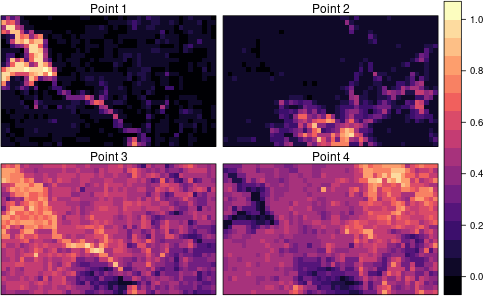
\includegraphics[width=\textwidth]{searchhis_plot2.png}
	\caption{Output similarity maps}
	\label{FIG:SEARCH2}
\end{figure}

\FloatBarrier

\subsubsection{Search on time series}
Figure \ref{FIG:SEARCHTS} presents general workflow path for producing similarity maps using a time-series raster data. 

\begin{figure}[H]
	\centering
	\includegraphics[width=\textwidth]{searchts_scheme.png}
	\caption{Workflow path for search on time series}
	\label{FIG:SEARCHTS}
\end{figure}

The first step is to prepare signature files for both, grid of motifels and query motifels, using two separate modules, {\tt gpat\_gridts} and {\tt gpat\_pointsts} respectively. 
The second step is to use these signature files as inputs to {\tt gpat\_search} module in order to the produce similarity maps.\\\\

{\bf Example:}

\begin{minipage}{\linewidth}
\begin{lstlisting}
gpat_gridts -i GB_pr01.tif -i GB_pr02.tif -i GB_pr03.tif -i GB_pr04.tif -i GB_pr05.tif -i GB_pr06.tif -i GB_pr07.tif -i GB_pr08.tif -i GB_pr09.tif -i GB_pr10.tif -i GB_pr11.tif -i GB_pr12.tif -o GB_pr_grid -n
gpat_pointsts -i GB_pr_grid -o query_signatures_ts.txt --xy_file=coordinates_gb.txt
gpat_search -i GB_pr_grid -r query_signatures_ts.txt -m tsEUC
\end{lstlisting}
\end{minipage}

For example, we want to find out which cities in Great Britain have the most (and the least) similar temporal pattern of precipitation. 
For this purpose, we need to have maps of precipitation (e.g. twelve rasters with monthly sums of precipitation from January to December) and coordinates of our points of interest (Figure \ref{FIG:SEARCHTS1}).

\newpage

\begin{wrapfigure}{l}{0.35\textwidth}
	\includegraphics[width=0.33\textwidth]{searchts_plot1.png}
	\caption{Location of the points of interest}
	\label{FIG:SEARCHTS1}
\end{wrapfigure}

Firstly, a grid which contains temporal patterns of precipitation need to be built based on the precipitation rasters.
Secondly, query signatures are extracted based on the coordinates of points of interest - in our case cities of London, Glasgow, Cardiff, Fort William, and Dublin. Finally, we can create the maps of similarity (one for each city). 
To do so, we need to specify the similarity measure proper for time series data, such as {\it tsEUC} (time series - euclidean distance).
Our final five maps show where the annual precipitation patterns are the most and the least similar to those in our selected cities (Figure \ref{FIG:SEARCHTS2}). \\\\\\\\\\

\begin{figure}[H]
        \begin{center}
	\includegraphics[width=0.75\textwidth]{searchts_plot2.png}
	\caption{Maps of the similarity in terms of precipitation time-series}
	\label{FIG:SEARCHTS2}
        \end{center}
\end{figure}

\FloatBarrier

\subsection{Change detection}

Change detection module provides a way to compare patterns between two grids-of-scenes.
The output map show the level of similarity between two inputs.
Figure \ref{FIG:CHANGE} presents general workflow path for producing maps of change. 

\begin{figure}[H]
	\centering
	\includegraphics[width=\textwidth]{compare_scheme.png}
	\caption{Workflow path for change detection}
	\label{FIG:CHANGE}
\end{figure}

The first step is to prepare signature files for both dataset, using either {\tt gpat\_gridhis} for categorical data or {\tt gpat\_gridts} for time series data.
The second step is to use these signature files as inputs to the {\tt gpat\_compare} module in order to the produce change maps. \\\\

{\bf Example:}

\begin{minipage}{\linewidth}
\begin{lstlisting}
gpat_gridhis -i Augusta2006.tif -o Augusta2006_grid100 -z 100 -f 100
gpat_gridhis -i Augusta2011.tif -o Augusta2011_grid100 -z 100 -f 100
gpat_compare -i Augusta2006_grid100 -i Augusta2011_grid100 -o Augusta0611_compared.tif
\end{lstlisting}
\end{minipage}

For example, we want to compare a change in land cover patterns between years 2006 and 2011. 
For this purpose, we can use a land cover data from NLCD for 2006 and 2011 (Figure \ref{FIG:CHANGEDET1}).
Both of these datafiles need to have the same extent and resolution.

Firstly, we need to create a grid of signatures for both GeoTIFF files.
It is important to remember that both of the created grid of signatures must by created using the same size, shift, and signature.

\begin{figure}[H]
	\centering
	\includegraphics[width=\textwidth]{change_det_two_maps.png}
	\caption{Land cover maps of Augusta for year 2006 and 2011}
	\label{FIG:CHANGEDET1}
\end{figure}

Secondly, the output map is created based on the grids of signatures.
The final map shows where a land cover pattern stayed the same (value of 1) and where it changed. 
The lowest values indicate the biggest change of a land cover pattern.

\begin{figure}[H]
	\centering
	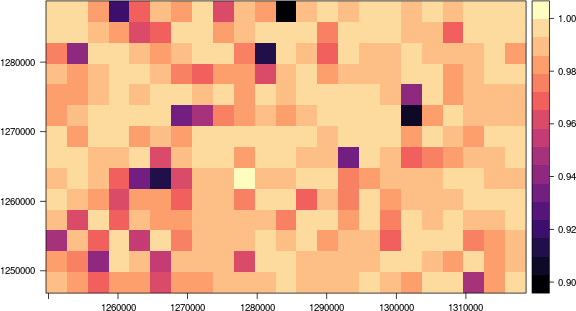
\includegraphics[width=\textwidth]{change_det.png}
	\caption{Maps of the similarity between a land cover of Augusta between 2006 and 2011}
	\label{FIG:CHANGEDET2}
\end{figure}

\FloatBarrier

\subsection{Segmentation \label{segmentation}}

Segmentation module enables user to create maps of segments.
Each of the output segment is internally homogeneous in terms of encapsulated pattern and, at the same time, different from the adjacent segments.
The input is a grid of signatures.
The result is a raster (GeoTIFF) and vector (ESRI Shapefile) file containing the segments.
Quality of segmentation could be also determined with raster maps of inhomogeneity, isolation, and overall quality.
Figure \ref{FIG:SEGMENT} presents general workflow path for segmentation. 

\begin{figure}[H]
	\centering
	\includegraphics[width=\textwidth]{segment_scheme.png}
	\caption{Workflow path for segmentation}
	\label{FIG:SEGMENT}
\end{figure}

\subsubsection{Segmentation on categorical maps}

{\bf Example:}

\begin{minipage}{\linewidth}
\begin{lstlisting}
gpat_gridhis -i Augusta2011.tif -o Augusta2011_grid100 -z 100 -f 100
gpat_segment -i Augusta2011_grid100 -o Augusta2011_seg100.tif -v Augusta2011_seg100.shp  --lthreshold=0.1 --uthreshold=0.3
gpat_segquality -i Augusta2011_grid100 -s Augusta2011_seg100.tif -g Augusta2011_seg100_ih.tif -o Augusta2011_seg100_is.tif
\end{lstlisting}
\end{minipage}

The first step is to prepare a signature file for the dataset, using the {\tt gpat\_gridhis} module.
The second step is to use this signature file as input to the {\tt gpat\_segment} module in order to the produce a segmentation map. 
The third, optional, step is to determine a quality of segmentation using the {\tt gpat\_segquality} module.\\\\

\newpage

For example, we want to find and delineate areas of similar land cover patterns. 

Firstly, we need to create a grid of signatures. 
Several options could be specified, such as the size and shift, type of motifel's signature, and normalization method.
Values of size and shift could be used to delineate patterns in different spatial scale, while the motifel's signature type and normalization method need to be selected based on the output data type.
We want to create segments with a spatial scale of six kilometers. 
To do so, we must to set adequate size and shift. 
As a default, segmentation process uses the brick topology, in which rectangular areas are merged to create each brick.
Therefore, to create segments with a spatial scale of six kilometers (area of 36 sq km), we need to set both size and shift to 100.
It is because one cell has resolution of 30 meters, and firstly using {\tt gpat\_gridhis} it is combined into a grid of signature of 3 kilometers (30 meters x 100 = 3 kilometers), and secondly using {\tt gpat\_segment} it is merged into bricks of four grids of signatures (6 by 6 kilometers). 
% See Appendix \ref{topology} for the details.
We left the rest of the parameters to the default values, with the signature in form of spatial coocurrence of the categories and the pdf normalization.

Secondly, the output of the previous step is used for segmentation. 
There we can modify several parameters of segmentation, such as the similarity measure, and minimum and maximum distance threshold to build areas.
The threshold values could be used to control a number of final segments.
As a result, we get the output segmentation as a raster (GeoTIFF) and vector (ESRI Shapefile) (Figure \ref{FIG:SEG1}).

\begin{figure}[H]
	\centering
	\includegraphics[width=\textwidth]{augusta2011_seg.png}
	\caption{Segments of land cover patterns of the 6km scale for Augusta}
	\label{FIG:SEG1}
\end{figure}

\begin{figure}[H]
	\centering
	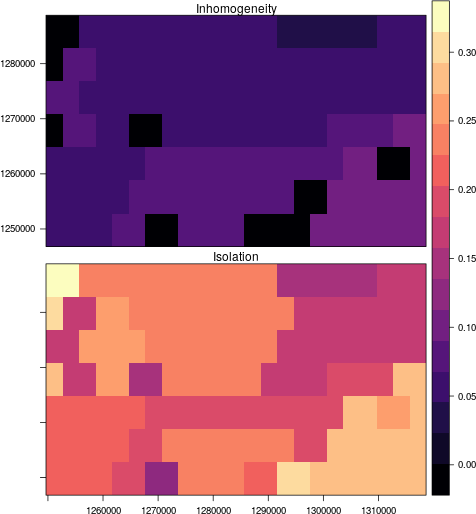
\includegraphics[width=\textwidth]{segmentation_quality.png}
	\caption{Inhomogenety and isolation metrics for the segmentation output}
	\label{FIG:SEG2}
\end{figure}

We can evaluate the quality of a segmentation using two metrics - inhomogeneity and isolation (Figure \ref{FIG:SEG2}).
Inhomogeneity indicates how much each segment is internally diverse (lower is better).
Isolation shows how much each segment is different from theirs neighbors (higher is better). 
Based on these two raster, it is possible to calculate the segmentation quality raster ($quality = 1 - (inhomogeneity/isolation)$) (higher is better; Figure \ref{FIG:SEG3}).
We can also calculate the overall quality as an average quality of all the segments.
In this example it is 0.82.

\begin{figure}[H]
	\centering
	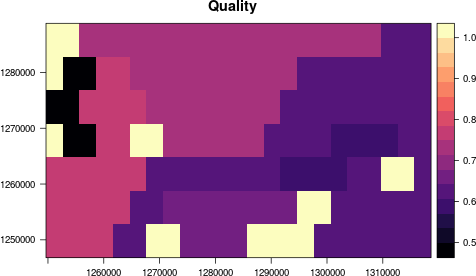
\includegraphics[width=\textwidth]{segmentation_qualityall.png}
	\caption{Quality of the segmentation of land cover patterns}
	\label{FIG:SEG3}
\end{figure}

\FloatBarrier

\subsubsection{Segmentation on time series}

{\bf Example:}

\begin{minipage}{\linewidth}
\begin{lstlisting}
gpat_gridts -i GB_pr01.tif -i GB_pr02.tif -i GB_pr03.tif -i GB_pr04.tif -i GB_pr05.tif -i GB_pr06.tif -i GB_pr07.tif -i GB_pr08.tif -i GB_pr09.tif -i GB_pr10.tif -i GB_pr11.tif -i GB_pr12.tif -o GB_pr_grid -n
gpat_segment -i GB_pr_grid -o GB_pr_seg.tif -v GB_pr_seg.shp -m tsEUC --lthreshold=0.5 --uthreshold=1
gpat_segquality -i GB_pr_grid -s GB_pr_seg.tif -g GB_pr_seg_ih.tif -o GB_pr_seg_is.tif -m tsEUC
\end{lstlisting}
\end{minipage}

The first step is to prepare a signature file for the dataset, using the {\tt gpat\_gridts} module.
The second step is to use this signature file as input to the {\tt gpat\_segment} module in order to the produce a segmentation map. 
The third, optional, step is to determine a quality of segmentation using the {\tt gpat\_segquality} module.\\\\

\newpage

\begin{wrapfigure}{r}{0.5\textwidth}
	\centering
	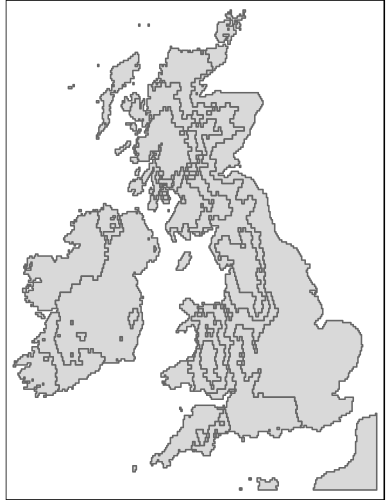
\includegraphics[width=0.4\textwidth]{ts_seg.png}
	\caption{Segments of the monthly precipitation temporal patterns for Great Britain}
	\label{FIG:SEGTS1}
\end{wrapfigure}

For example, we want to find and delineate areas of similar time-series patterns of precipitation in Great Britain. 

Firstly, we need to create a grid of signatures using twelve raster with monthly average values of precipitation.
Depending on the input data it could be important to normalize data using the {\it --normalize} option.

Secondly, the output of the previous step is used for segmentation.
As a result, we get the output segmentation as a raster (GeoTIFF) and vector (ESRI Shapefile) (Figure \ref{FIG:SEGTS1}).

We can evaluate the quality of a segmentation using two metrics - inhomogeneity and isolation (Figure \ref{FIG:SEGTS2}).
Based on these two raster, it is possible to calculate the segmentation quality raster (Figure \ref{FIG:SEGTS3}).
We can also calculate the overall quality as an average quality of all the segments.
In this example it is 0.67.

\begin{figure}[H]
	\centering
	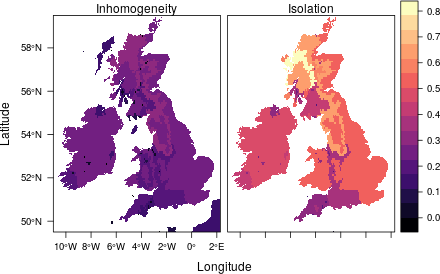
\includegraphics[width=\textwidth]{ts_segmentation_ihis.png}
	\caption{Inhomogenety and isolation metrics for the segmentation of the monthly precipitation temporal patterns for Great Britain}
	\label{FIG:SEGTS2}
\end{figure}

\begin{figure}[H]
	\centering
	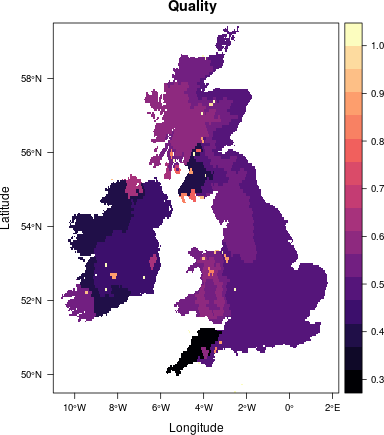
\includegraphics[width=\textwidth]{ts_segmentation_qualityall.png}
	\caption{Quality of the segmentation of the monthly precipitation temporal patterns for Great Britain}
	\label{FIG:SEGTS3}
\end{figure}

\FloatBarrier

\subsection{Clustering \label{clustering}}

Clustering module enables users to create distance matrices, which can be later used in a statistical software (such as R) to perform a clustering.
Distance matrix can be created for selected motifels, a grid of motifels, and predefined regions (e.g. segments).

Examples in this section are using R (\cite{R}) for a clustering and visualization of the results. 
They require the latest versions of R (\url{https://cloud.r-project.org/}) and a set of packages installed by executing the below code in R:

\begin{minipage}{\linewidth}
\lstset{backgroundcolor=\color{antiflashwhite}}
\begin{lstlisting}
install.packages("sf")
install.packages("tmap")
install.packages("devtools")
devtools::install_github("nowosad/rgeopat2")
\end{lstlisting}
\end{minipage}

\subsubsection{Clustering of individual motifels}

\begin{figure}[H]
	\centering
	\includegraphics[width=\textwidth]{cluster_points_scheme.png}
	\caption{Workflow path for a clustering of motifels}
	\label{FIG:CLUSTER_POINTS}
\end{figure}

The first step is to prepare a signature file for query motifels using the {\tt gpat\_pointsts} module. 
The second step is to calculate a distance matrix based on a selected similarity measure using {\tt gpat\_distmtx} (Figure \ref{FIG:CLUSTER_POINTS}).

{\bf Example:}

\begin{minipage}{\linewidth}
\begin{lstlisting}
gpat_pointshis -i Augusta2011.tif -o Augusta2011_selected.txt  -s cooc -z 50 -n pdf --xy_file=Augusta2011_sel_points.txt
gpat_distmtx -i Augusta2011_selected.txt -o Augusta2011_matrix.csv
\end{lstlisting}
\end{minipage}

For example, we create signatures based on a given size (e.g. 50) and signature type for selected motifels using a text file with the coordinates of points of interest.
Next, we calculate distances between all of these motifels using selected similarity measure (in this example, we used the default one - 'jsd' Jensen-Shannon Divergence).

Created distance matrix can be used in R:

\begin{minipage}{\linewidth}
\lstset{backgroundcolor=\color{antiflashwhite}}
\begin{lstlisting}
library(rgeopat2)
dist_matrix = gpat_read_distmtx("Augusta2011_matrix.csv")
hclust_result = hclust(d = dist_matrix, method = "ward.D2")
plot(hclust_result, labels = FALSE)
sel_points = read.csv("Augusta2011_sel_points.txt", header = FALSE) 
sel_points$class = cutree(hclust_result, k = 5)
plot(augusta2011)
points(sel_points, pch = 20, cex = 3, col = sel_points$class)
\end{lstlisting}
\end{minipage}

The {\tt gpat\_read\_distmtx} function reads a distance matrix from a file. 
Next, this file is used for a clustering. 
There are several clustering methods in R that accept a distance matrix as an input, such as hierarchical clustering ({\tt hclust}) and partitioning around medoids ({\tt cluster::pam}).
Here, we use and visualize a result of hierarchical clustering (left panel of figure \ref{FIG:CLUSTER_POINTS2}).
Based on the dendrogram, data is divided into five groups and the information about class numbers is added to the object containing our selected points.
Finally, we visualize the results (right panel of figure \ref{FIG:CLUSTER_POINTS2}).

\begin{figure}[H]
  \begin{subfigure}[b]{0.5\textwidth}
    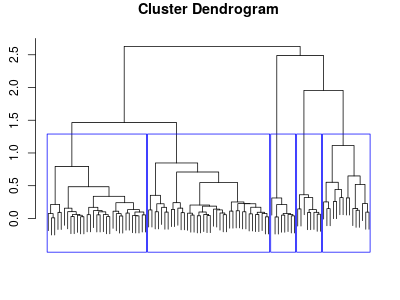
\includegraphics[width=\textwidth]{clustering_example_motifels_his1.png}
    \label{FIG:CLUSTER_POINTS2a}
  \end{subfigure}
  \begin{subfigure}[b]{0.5\textwidth}
    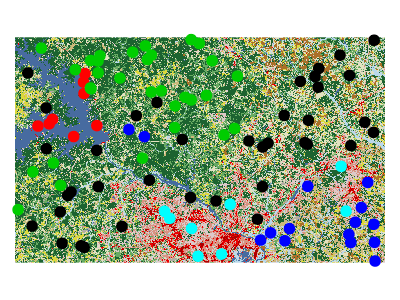
\includegraphics[width=\textwidth]{clustering_example_motifels_his2.png}
    \label{FIG:CLUSTER_POINTS2b}
  \end{subfigure}
  \caption{Example of a clustering of motifels}
  \label{FIG:CLUSTER_POINTS2}
\end{figure}

\begin{figure}[H]
	\centering
	\includegraphics[width=\textwidth]{cluster_pointsts_scheme.png}
	\caption{Workflow path for a clustering of time series motifels}
	\label{FIG:CLUSTER_POINTSTS}
\end{figure}

Procedure for time-series data is slightly different (Figure \ref{FIG:CLUSTER_POINTSTS}).
The first step is to create a signature grid file using a time-series of rasters using the {\tt gpat\_gridts} module.
The second step is to extract only selected motifels using {\tt gpat\_pointsts}.
The third step is to calculate and export a distance matrix with {\tt gpat\_distmtx}.

{\bf Example:}

\begin{minipage}{\linewidth}
\begin{lstlisting}
gpat_gridts -i GB_pr01.tif -i GB_pr02.tif -i GB_pr03.tif -i GB_pr04.tif -i GB_pr05.tif -i GB_pr06.tif -i GB_pr07.tif -i GB_pr08.tif -i GB_pr09.tif -i GB_pr10.tif -i GB_pr11.tif -i GB_pr12.tif -o GB_pr_grid -n
gpat_pointsts -i GB_pr_grid -o GB_pr_points.txt --xy_file=GB_cities.csv
gpat_distmtx -i GB_pr_points.txt -o GB_pr_distmat.csv -m tsEUC 
\end{lstlisting}
\end{minipage}

For example, we want to find cities in Great Britain with very similar temporal patterns of a monthly sum of precipitation. 
For this purpose, we need to have twelve rasters with values of a monthly sum of precipitation for the whole area of Great Britain and the list of the cities coordinates (the GB\_cities.csv file).
Firstly, we can create a signature grid. 
Next step is to extract the signature only for the locations in our GB\ cities.csv file.
Finally, we can calculate and export distance matrix using euclidean distance {\it tsEUC}.

Created distance matrix can be used in R:

\begin{minipage}{\linewidth}
\lstset{backgroundcolor=\color{antiflashwhite}}
\begin{lstlisting}
library(sf)
library(tmap)
library(rgeopat2)
dist_matrix = gpat_read_distmtx("GB_pr_distmat.csv")
hclust_result = hclust(d = dist_matrix, method = "ward.D2")
plot(hclust_result, labels = FALSE)
sel_points = read.csv("GB_cities.csv", header = FALSE) 
sel_points$class = as.factor(cutree(hclust_result, k = 4))
sel_points_st = st_as_sf(sel_points, coords = c("V1", "V2"))
tm_shape(british_isles) +
        tm_polygons() +
        tm_shape(sel_points_st) +
        tm_dots(col = "class", size = 0.25, title = "Class: ")
\end{lstlisting}
\end{minipage}

The {\tt gpat\_read\_distmtx} function reads a distance matrix from a file. 
Next, we use and visualize a result of hierarchical clustering (left panel of figure \ref{FIG:CLUSTER_POINTSTS2}).
Based on the dendrogram, data is divided into four groups and the information about class numbers is added to the object containing our selected points.
Using the {\tt st\_as\_sf} function, we transform our selected points into spatial object.
Finally, we visualize the results using functions from the {\tt tmap} package (right panel of figure \ref{FIG:CLUSTER_POINTS2}).
For this purpose, we use a map of British Isles {\it british\_isles} from the {\tt rgeopat2} package and the spatial object with our selected points ({\it sel\_points\_st}).

\begin{figure}[H]
  \begin{subfigure}[b]{0.5\textwidth}
    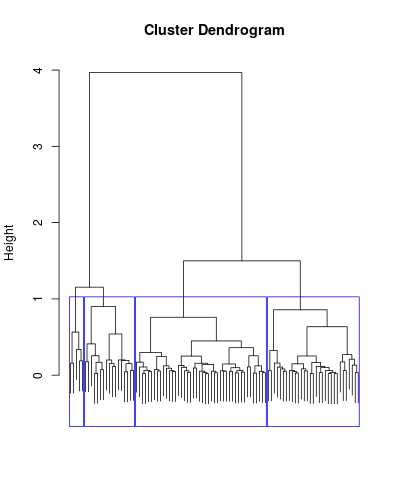
\includegraphics[width=\textwidth]{clustering_example_motifels_ts1.png}
  \end{subfigure}
  \begin{subfigure}[b]{0.5\textwidth}
    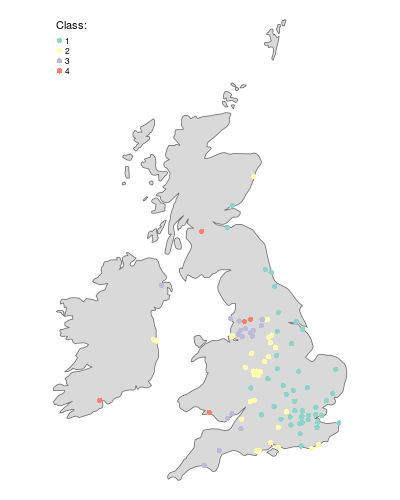
\includegraphics[width=\textwidth]{clustering_example_motifels_ts2.png}
  \end{subfigure}
  \caption{Example of a clustering of time series motifels}
  \label{FIG:CLUSTER_POINTSTS2}
\end{figure}

\FloatBarrier

\subsubsection{Clustering of a grid of motifels}

\begin{figure}[H]
	\centering
	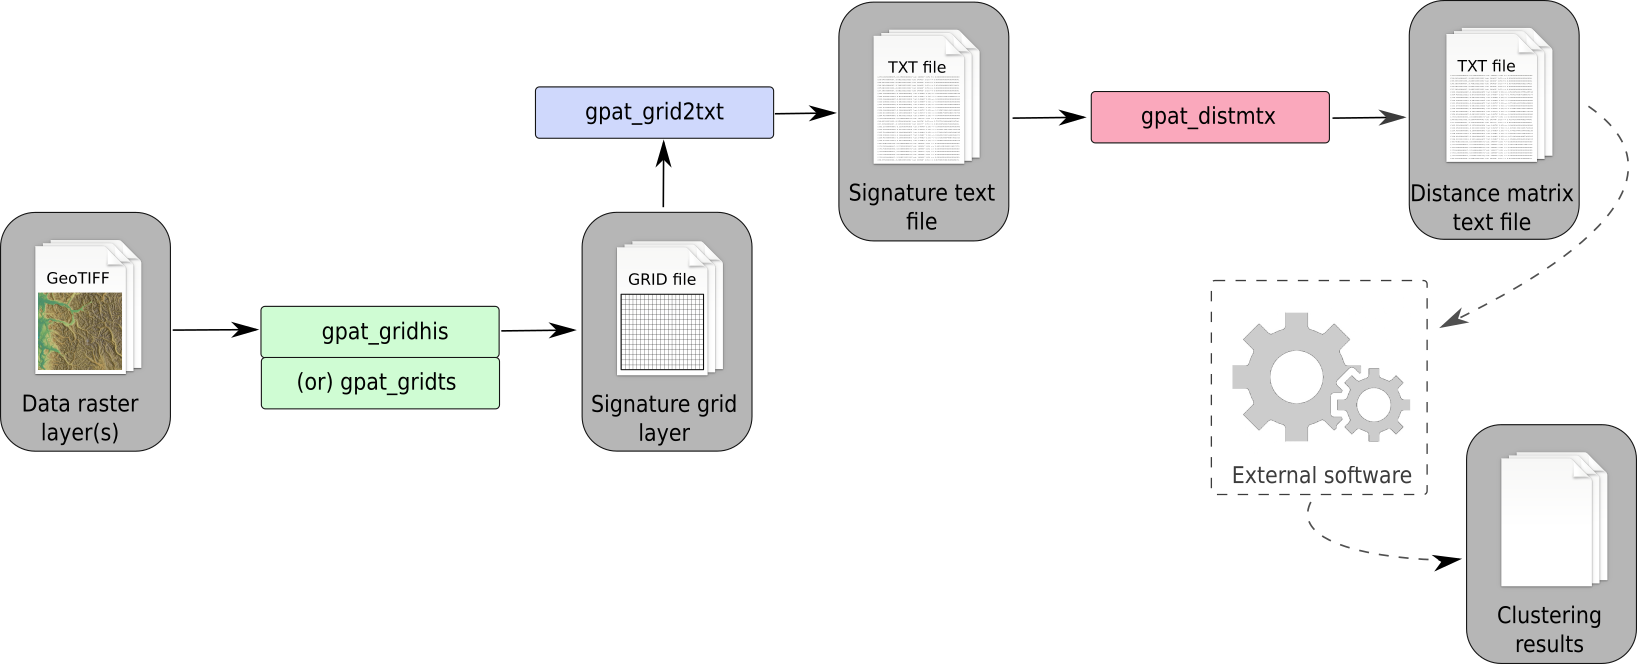
\includegraphics[width=\textwidth]{cluster_grid_scheme.png}
	\caption{Workflow path for a clustering of a grid of motifels}
	\label{FIG:CLUSTER_GRID}
\end{figure}

The first step is to create a signature grid using either the {\tt gpat\_gridhis} or {\tt gpat\_gridts} module.
The second step is to convert the obtained signature grid from binary to text format with {\tt gpat\_grd2txt}.
The final step is to calculate and export a distance matrix using the {\tt gpat\_distmtx} module (Figure \ref{FIG:CLUSTER_GRID}).

{\bf Example:}

\begin{minipage}{\linewidth}
\begin{lstlisting}
gpat_gridhis -i Augusta2011.tif -o Augusta2011_grid100 -z 100 -f 100
gpat_grd2txt -i Augusta2011_grid100 -o Augusta2011_grid100.txt
gpat_distmtx -i Augusta2011_grid100.txt -o Augusta2011_matrix_grid.csv
\end{lstlisting}
\end{minipage}

For example, we want to find groups of areas with similar pattern of a land cover in scale of 3 kilometers.
Firstly, we need to calculate a signature grid with the size and shift options set to 100 (30 meters resolution multiplied by 100 is 3 kilometers).
Next, we convert the signature grid to a text file.
This new file will be an output to for the calculations of a distance matrix.
A default similarity measure, Jensen-Shannon divergence, can be used here, as it is suitable for a land cover data.

Created distance matrix can be used in R:

\begin{minipage}{\linewidth}
\lstset{backgroundcolor=\color{antiflashwhite}}
\begin{lstlisting}
library(sf)
library(rgeopat2)
dist_matrix = gpat_read_distmtx("Augusta2011_matrix_grid.csv")
hclust_result = hclust(d = dist_matrix, method = "ward.D2")
plot(hclust_result, labels = FALSE)
hclust_cut = cutree(hclust_result, 5)
my_grid = gpat_gridcreate("Augusta2011_grid100.hdr")
my_grid$class = hclust_cut
plot(my_grid)
\end{lstlisting}
\end{minipage}

The {\tt gpat\_read\_distmtx} function reads a distance matrix from a file. 
Next, we use and visualize a result of hierarchical clustering (left panel of figure \ref{FIG:CLUSTER_GRID2}).
Based on the dendrogram, data is divided into five groups and the information about class numbers is added to the object containing our selected points.
Using the {\tt gpat\_gridcreate} function, we create a new grid polygon and add the class numbers to it.
Finally, we visualize the results (right panel of figure \ref{FIG:CLUSTER_GRID2}).

\begin{figure}[H]
  \begin{subfigure}[b]{0.5\textwidth}
    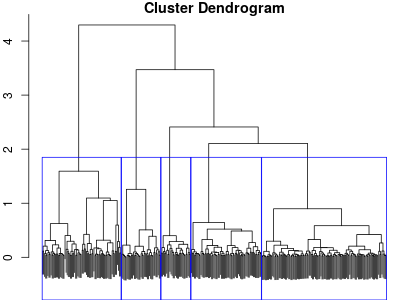
\includegraphics[width=\textwidth]{clustering_example_grid1.png}
  \end{subfigure}
  \begin{subfigure}[b]{0.5\textwidth}
    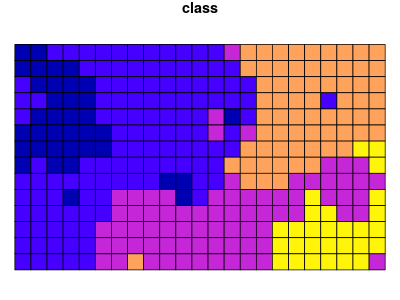
\includegraphics[width=\textwidth]{clustering_example_grid2.png}
  \end{subfigure}
  \caption{Example of a clustering of a grid of motifels}
  \label{FIG:CLUSTER_GRID2}
\end{figure}

\FloatBarrier

\subsubsection{Clustering of segments / predefined irregular regions}

\begin{figure}[H]
	\centering
	\includegraphics[width=\textwidth]{cluster_seg_scheme.png}
	\caption{Workflow path for a clustering of segments (regions)}
	\label{FIG:CLUSTER_SEGMENT}
\end{figure}

The first step is to unify the resolution and extent of the input raster data and the segment file, which can be done using a GIS software, such example {\tt gdalwrap}.
The second step is to calculate the signature file based on a raster data which contain a pattern to analyze and a raster data with segments (or any other irregular regions) using the {\tt gpat\_polygon} module.
The third step is to create and export a distance matrix using {\tt gpat\_distmtx} (Figure \ref{FIG:CLUSTER_SEGMENT}).

{\bf Example:}

\begin{minipage}{\linewidth}
\begin{lstlisting}
gdalwarp -tr 30 30 Augusta2011_seg100.tif Augusta2011_seg100_res.tif
gpat_polygon -i Augusta2011.tif -e Augusta2011_seg100_res.tif -o Augusta2011_psign.txt
gpat_distmtx -i Augusta2011_psign.txt -o Augusta2011_matrix_seg.csv
\end{lstlisting}
\end{minipage}

For example, in the section \ref{segmentation} we created segments with homogeneous patterns of land cover.
Now we can find and group similar non-adjacent segments with clustering.
Firstly, we need to change the resolution of the segment file to 30 meters (this is the resolution of the land cover data).
Next, we need to create a signature text file for each of the segments.
Based on the new file we can calculate a distance between each pair of the segments using selected dissimilarity metric, such as Jensen-Shannon divergence.

Created distance matrix can be used in R:

\begin{minipage}{\linewidth}
\lstset{backgroundcolor=\color{antiflashwhite}}
\begin{lstlisting}
library(sf)
library(rgeopat2)
dist_matrix = gpat_read_distmtx("Augusta2011_matrix_seg.csv")
hclust_result = hclust(d = dist_matrix, method = "ward.D2")
plot(hclust_result, label = FALSE)
hclust_cut = cutree(hclust_result, 3)
segm = st_read("Augusta2011_seg100.shp")
segm$class = hclust_cut
plot(segm["class"])
\end{lstlisting}
\end{minipage}

The {\tt gpat\_read\_distmtx} function reads a distance matrix from a file. 
Next, we use and visualize a result of hierarchical clustering (left panel of figure \ref{FIG:CLUSTER_SEGMENT2}).
Based on the dendrogram, data is divided into three groups and the information about class numbers is added to the object containing our selected points.
Using the {\tt st\_read} function, we read our polygons into R and add the class number to each polygon.
Finally, we visualize the results (right panel of figure \ref{FIG:CLUSTER_SEGMENT2}).

\begin{figure}[H]
  \begin{subfigure}[b]{0.5\textwidth}
    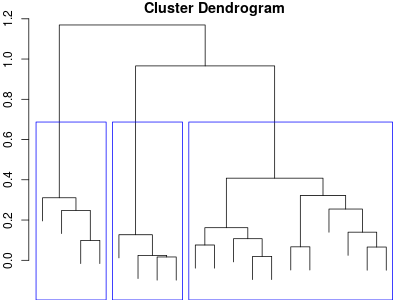
\includegraphics[width=\textwidth]{clustering_example_polygon1.png}
  \end{subfigure}
  \begin{subfigure}[b]{0.5\textwidth}
    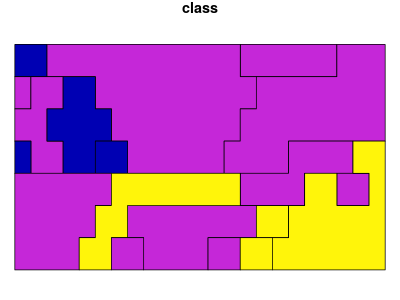
\includegraphics[width=\textwidth]{clustering_example_polygon2.png}
  \end{subfigure}
  \caption{Example of a clustering of a grid of segments (regions)}
  \label{FIG:CLUSTER_SEGMENT2}
\end{figure}


\newpage
